\documentclass[UTF8]{ctexart}
\usepackage{boxedminipage}
\usepackage{float}
\usepackage{hyperref}
\usepackage{graphicx}
\usepackage{multirow}
%================样式================
\usepackage[\VAR{geometry.header}]{geometry}
\setlength{\headsep}{\VAR{geometry.headsep}mm}
%\usepackage{setspace}
%\setstretch{1}
\usepackage{enumitem}
\setenumerate[1]{partopsep=0mm,parsep=\parskip,topsep=0mm}
%================交叉引用================
\renewcommand{\figureautorefname}{图}
%================快捷,与Python程序无关================
\newcommand{\smalltitle}[1]{{\zihao{4}\bfseries{#1}}\\} 
%================页眉================
\usepackage{fancyhdr}
\usepackage{lastpage}
\pagestyle{fancy}
\renewcommand{\headrulewidth}{0.5pt}
%\renewcommand{\footrulewidth}{0pt}
\fancyhf{}
\setlength{\headheight}{\VAR{geometry.headheight}mm}
\chead{
\centering
{\zihao{3}\textbf{生产作业指导书}}\\\medskip
\zihao{5}
\setlength{\tabcolsep}{\VAR{htable.tabcolsep}mm}
\begin{tabular}{|c|c|c|c|c|}
\hline
\VAR{htable.mcr("产品名称",(1,2),2,"l")}&
%\VAR{htable.cell("产品件号",2)}&
\VAR{htable.cell("设备名称",3)}&
\VAR{htable.cell("设备编号",4)}&
\VAR{htable.cell("使用阶段",5)}\\
\hline
%\VAR{htable.cell("见\\textless 适用产品清单 \\textgreater",1)}&
%\VAR{htable.cell("见\\textless 适用产品清单 \\textgreater",2)}&
\VAR{htable.mcrb((1,2))}&
\VAR{htable.cell("输入轴、扭杆压机",3)}&
\VAR{htable.cell("569-701077",4)}&\VAR{htable.cell("",5)}\\
\hline
\VAR{htable.cell("工序号",1)}&
\VAR{htable.cell("工序名称",2)}&
\VAR{htable.cell("编制日期",3)}&
\VAR{htable.cell("版本号",4)}&
\VAR{htable.cell("页数",5)}\\
\hline
\VAR{htable.cell("OP30/40",1)}&
\VAR{htable.cell("蜗轮轴压扭杆/输入轴压自润滑衬套",2)}&
\VAR{htable.cell("2020.5.14",3)}&
\VAR{htable.cell("B01",4,"c","b")}&
\VAR{htable.cell("第\\thepage 页,共\\pageref{LastPage}页",5)}\\
\hline
\end{tabular}\\
}
%================正文的环境设置================
\begin{document}
\zihao{5}
\centering
%================正文内容================
\begin{boxedminipage}{\VAR{geometry.textwidth|round(2)}mm}
\centering
\smalltitle{开班准备描述}
\begin{boxedminipage}[t]{\VAR{geometry.intro_width|round(2)}mm}
\begin{enumerate}
\BLOCK{for i in 开班准备描述}
\item \VAR{i}
\BLOCK{endfor}
\end{enumerate}
\end{boxedminipage}
\hfill
\begin{boxedminipage}[t]{\VAR{geometry.picbox_width|round(2)}mm}
\begin{figure}[H]
\parbox[t]{\VAR{geometry.picbox_half_width|round(2)}mm}{
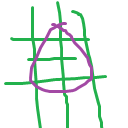
\includegraphics[width=\VAR{geometry.picbox_half_width|round(2)}mm]{pic01}
\caption{}}
\hfill
\parbox[t]{\VAR{geometry.picbox_half_width|round(2)}mm}{
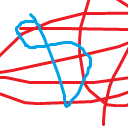
\includegraphics[width=\VAR{geometry.picbox_half_width|round(2)}mm]{pic02}
\caption{}}
\end{figure}
\end{boxedminipage}
\end{boxedminipage}
\begin{boxedminipage}{\VAR{geometry.textwidth|round(2)}mm}
\centering
\smalltitle{设备开机描述}
\begin{boxedminipage}[t]{\VAR{geometry.intro_width|round(2)}mm}
\begin{enumerate}
\BLOCK{for i in 设备开机描述}
\item \VAR{i}
\BLOCK{endfor}
\end{enumerate}
\end{boxedminipage}
\hfill
\begin{boxedminipage}[t]{\VAR{geometry.picbox_width|round(2)}mm}
图片2
\end{boxedminipage}
\end{boxedminipage}
\end{document}